\documentclass[10pt,xcolor={svgnames}]{beamer}

%%%%% Colors
\usetheme{Dresden}%\usetheme{Madrid}
\colorlet{beamer@blendedblue}{green!55!black}
%%%%%

%%%%% Other 
\addtobeamertemplate{navigation symbols}{}{%
    \usebeamerfont{footline}%
    \usebeamercolor[fg]{footline}%
    \hspace{1em}%
    \insertframenumber/\inserttotalframenumber
}
\usepackage{hyperref, url}

\definecolor{pine_green}{HTML}{007935}
\hypersetup{colorlinks,breaklinks,linkcolor=white,urlcolor=orange,citecolor=black}
\renewcommand\thefootnote{\textcolor{pine_green}{\arabic{footnote}}}
\setbeamercolor{alerted text}{fg=pine_green}

\usepackage{cancel}
\usepackage{multirow}
\setbeamertemplate{itemize subitem}{$\circ$}
%%%%%

%%%%% Greying out/invidible Slides
\setbeamercovered{invisible}
\setbeamercovered{%
  again covered={\opaqueness<1->{15}}}
  
%%%%%







%%%%% Footnotes and captions
%\usepackage[utf8]{inputenc}
\usepackage{caption}
\usepackage{comment}
\usepackage{wasysym}
\setbeamerfont{footnote}{size=\tiny}
\setbeamerfont{caption}{size=\tiny}
%\setbeamerfont{normal text}{size=\small}
\setbeamerfont{itemize/enumerate body}{size=\small}
\setbeamerfont{itemize/enumerate subbody}{size=\footnotesize}
%%%%%



%Information to be included in the title page:
\title[Connor Wiegand]{Intro to Economic Analysis: Microeconomics}
\subtitle{EC 201 - Day 3 Slides}
\author[EC 201]{Connor Wiegand}
\institute[]{Department of Economics - University of Oregon}
\date{4 October 2021}


\begin{document}

\frame{\titlepage}

\begin{frame}{Logistics}
    \begin{itemize}[<+->]
        \item Sign up for Cengage, intro homework due tonight at 11:59pm
        \item Official homework 1 due this Saturday at 11:59pm, covering last week's material
        \item Some news assignments posted, first one due Wednesday, October 13
    \end{itemize}
\end{frame}

\begin{frame}{Transitioning to a New Topic}
    \begin{itemize}[<+->]
        \item Last week we covered PPFs and OC
        \item Reading the book hopefully gave you insight into incentives and other economic thinking ideas that we will build throughout the term
        \item Now we will transition to talking about markets for good, starting with the consumer side
        \item While PPFs and (specifically) OC will be important frameworks to keep in mind, they are more or less not the bread and butter of introductory micro
        \begin{itemize}
            \item <4-> That being said, OC will implicitly be present throughout the quarter
        \end{itemize}
    \end{itemize}
\end{frame}

\begin{frame}{The Relationship Between Price and Quantity}
    \begin{itemize}
        \item Activity: How many iced coffees would you get for...
        \begin{table}[H]
            \centering
            \begin{tabular}{c|c}
                Price & Quantity \\
                \hline
                \$0 &\pause 18\\
                \$0.50 &\pause 10\\
                \$1 &\pause 8\\
                \$2 &\pause 4\\
                \$3 &\pause 2\\
                \$4 &\pause 1\\
                \$5 &\pause 0
            \end{tabular}
        \end{table}
    \end{itemize}
\end{frame}


\begin{frame}{Individual Demand Curve}
    \begin{itemize}
        \item This set of points can be used to establish my \underline{individual demand curve}
        \begin{center}
            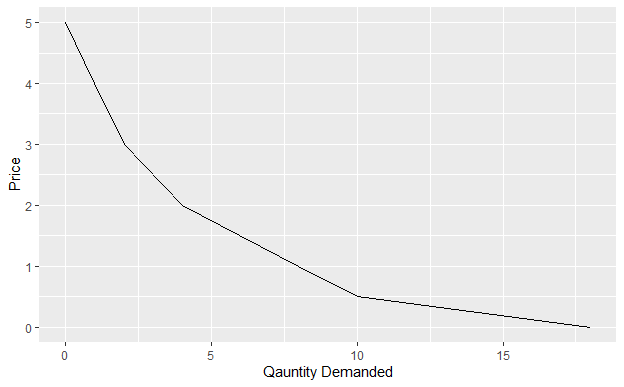
\includegraphics[width=10cm]{my demand curve.png}
        \end{center}
    \end{itemize}
\end{frame}

\begin{frame}{Market Demand}
    \begin{itemize}[<+->]
        \item Once we have multiple individual market demand curves, we can take their \textit{horizontal sum} to get market demand
        \begin{itemize}
            \item That is, if the market consists of 3 people, who each demand $q_{1}$, $q_{2}$, and $q_{3}$ iced coffees at a price of \$1, then the market demand for iced coffee at \$1 is $Q_{M}=q_{1}+q_{2}+q_{3}$
            \item
            \begin{center}
                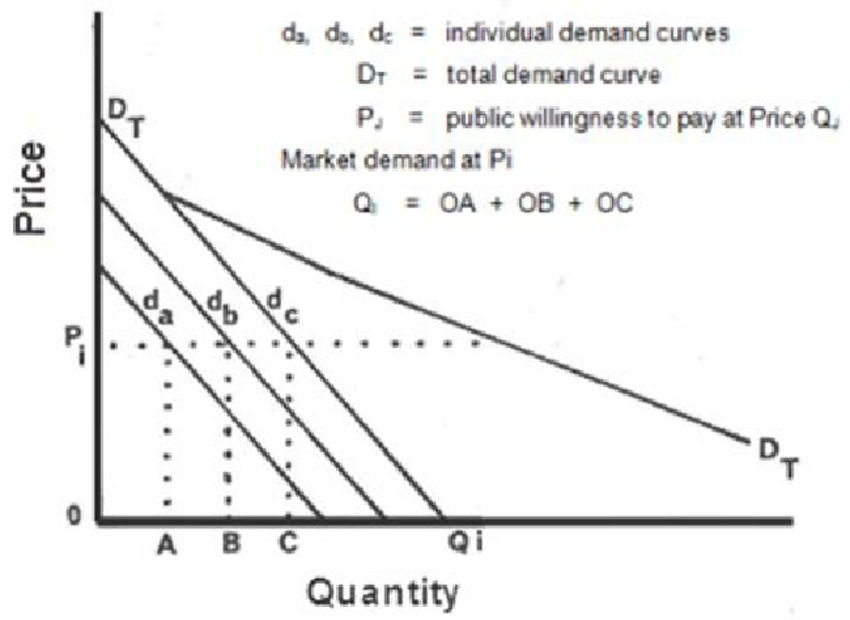
\includegraphics[width=7cm]{demand summing.png}
            \end{center}
        \end{itemize}
    \end{itemize}
\end{frame}

\begin{frame}{Market Demand Curve Example}
    \begin{itemize}[<+->]
        \item For example, if I am one member of the economy, and I have two of you as members of the economy, so that our three individual demand curves look like the this (left):
        \begin{table}[H]
            \centering
            \begin{tabular}{ll}
                \hspace{-18mm}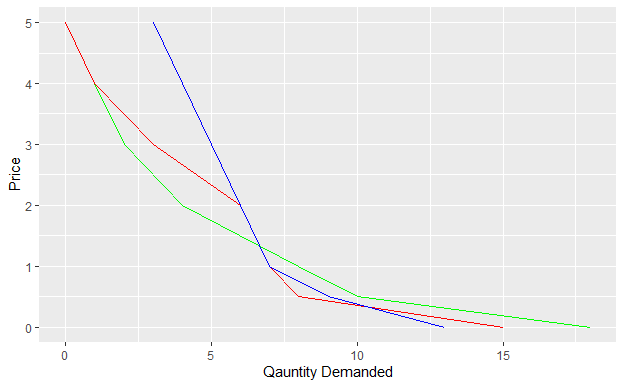
\includegraphics[width=6cm]{three i demands.png} & \pause 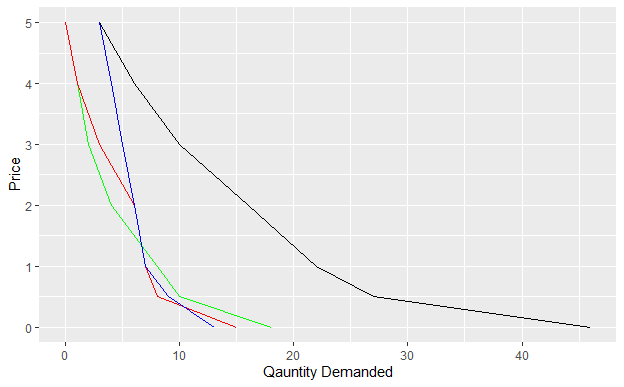
\includegraphics[width=6cm]{market demand.png}  
            \end{tabular}
        \end{table}
        \item<2-> Then our market demand will look like this (right)
    \end{itemize}
\end{frame}

\begin{frame}{Demand Curve Features}
    \begin{itemize}[<+->]
        \item What is the most obvious feature of the demand curve? 
        \begin{itemize}
            \item It's downward sloping
        \end{itemize}
        \item This says that the relationship between price and quantity demanded is negative: as the price goes up, you (or the market) demand less of the good in question
        \item This is formally known as the \underline{\textbf{Law of Demand}}: ``Other things being equal, when the price of a good rises, the quantity demanded of the good falls, and when the price falls, the quantity demanded rises"
    \end{itemize}
\end{frame}

\begin{frame}{Quick Aside}
    \begin{itemize}[<+->]
        \item The previous definition started with the phrase ``Other things being equal,"; you will also hear ``all else equal," or the latin phrase of similar meaning, ``ceteris paribus"\footnote{If you google the phrase and ask google to say it, it pronounces it with a hard ``kae", like in ``cater". However, if you google ``ceteris paribus pronunciation, google uses a soft ``seh". The former is regarded as correct while latter has been more common historically.\vspace{2mm}}
        \item This is an important theme in economics and general modelling (recall the map-maker example): we do not want to consider too many things at once
        \begin{itemize}
            \item Dumb example: you arrogantly challenge your professor to a drinking contest to decide your grade. I drink my favorite red wine on a full stomach, you drink \$10 everclear after a bowl of salad. 
            \item Real example: you want to find the impact that time of year has on gas prices, so you decide to compare gas price averages across different months: Jan-Jan, Feb-Feb, etc. Your sample years are 2019 and 2020
        \end{itemize}
        \item This is the challenge of empiricists/econometricians: isolating effects so that the analysis reasonably has ``all else equal"
        \item Doing theory (what we are doing), we just assert it\vspace{1mm}
    \end{itemize}
\end{frame}

\begin{frame}{Specificity of Market}
\begin{itemize}[<+->]
    \item Note that the demand curve measures the demand for a good in the \textit{market}, a key feature of microeconomics
    \item However, we can of course seek out various levels of specificity when defining these goods
    \item Ex: Food \& Drinks $>$ Drinks $>$ Non-alcoholic drinks $>$ Morning Beverages $>$ Coffee $>$ Iced Coffee $>$ Starbucks Iced Coffee
    \item Each time we move to a different tier, we may expect different characteristics in the shape of the demand curve
    \item We may also expect general trends as we move to more specific levels, which is a topic for next chapter
    \item Economists will often not compare demand curves across these different tiers, but it is not out the question (for example, when studying a specific firm with few types of services, like Uber)
\end{itemize}
\end{frame}

\begin{frame}{Shape of the Demand Curve}
    \begin{itemize}[<+->]
        \item So we know that the demand curve is downward sloping
        \item The shape of the demand curve is usually draw either bowed inward or linear
        \item While you can think about why this might be, it actually doesn't bear too much concern to us -- just draw it linear or bowed in for convention's sake
        \item On the other hand, the slope of the demand curve is of great importance, and we will discuss further in the next chapter and beyond
        \item The biggest topic in this chapter relating to the demand curve will being shifting it, or moving along it
    \end{itemize}
\end{frame}

\begin{frame}{What Would Cause Market Demand Curve to Shift?}
    \begin{itemize}[<+->]
        \item Changes in...
        \item Tastes and preferences (or trends)
        \begin{itemize}
            \item If millions of people see a video of pig feed being made out of plastic, the demand for bacon will fall
        \end{itemize}
        \item Prices of related goods
        \begin{itemize}
            \item If the price of hot dogs rises, the demand for hot dog buns will fall
            \item As the price of coke rises, the demand for pepsi will rise as well
        \end{itemize}
        \item Income 
        \begin{itemize}
            \item If all of your incomes doubled, we may see a rise in the demand for Rainier 
            \item But, we may also see a drop in the demand for PBR
        \end{itemize}
        \item Number of buyers in the market
        \begin{itemize}
            \item As the number of senior citizens increases, the demand for electric scooters might rise
        \end{itemize}
        \item Expectations
        \begin{itemize}
            \item If you anticipate the price of gas to increase tomorrow, you will buy more gas today
        \end{itemize}
    \end{itemize}
\end{frame}

\begin{frame}{Relevant Terminology}
\underline{Prices of Related Goods:}
    \begin{itemize}[<+->]
        \item Two goods are called \underline{\textbf{substitutes}} an increase in the price of one good leads to an increase in the demand of the other
        \item Two goods are called \underline{\textbf{complements}} an increase in the price of one good leads to an decrease in the demand of the other
    \end{itemize}
    \pause 
\underline{Income:}
    \begin{itemize}[<+->]
        \item A good is called \underline{\textbf{normal}} if an increase in income leads to an increase in demanded for said good
        \item A good is called \underline{\textbf{inferior}} if an increase in income leads to a decrease in demand for said good
    \end{itemize}
\end{frame}

\begin{frame}{What Do These Demand Changes Look Like?}
    \begin{itemize}[<+->]
        \item When the demand curve rises, we say that the demand curve shifts...
        \begin{itemize}
            \item outward
            \item rightward
            \item upward
        \end{itemize}
        \item Any are fine, I would say outward or rightward are preferred
        \item When the demand curve falls, we say that the demand curve shifts...
        \begin{itemize}
            \item inward
            \item leftward
            \item downward
        \end{itemize}
        \item We also may just say that demand rises or falls\footnote{On a test or assignment, you should be \underline{very} clear on whether or not you mean a curve shift or a movement along the curve}
    \end{itemize}
\end{frame}

\begin{frame}{What Do these Demand Changes look like? (cont.)}
    \begin{itemize}
        \item An example of sloped demand curves shifting:
        \begin{center}
            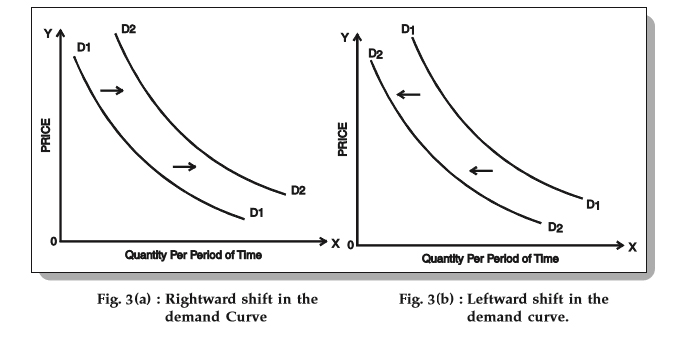
\includegraphics[width = 10cm]{demand shifts.jpg}
        \end{center}
        \item Note that shape and relative slope are preserved (later we may see examples where the slope can change)
    \end{itemize}
\end{frame}


\begin{frame}{What Do these Demand Changes look like? (cont.)}
    \begin{itemize}
        \item An example of linear demand curves shifting:
        \begin{center}
            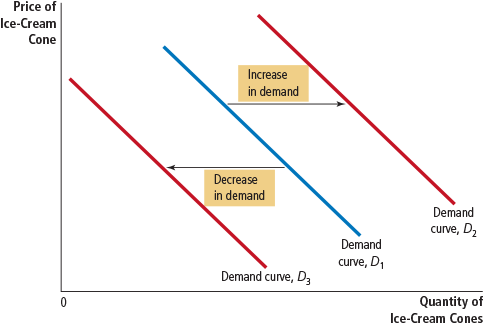
\includegraphics[width = 8cm]{demand shift.png}
        \end{center}
        \item Note the arrows and correct labelling 
    \end{itemize}
\end{frame}


\begin{frame}{Changes in Price}
    \begin{itemize}
        \item So our shifters of demand are
        \begin{itemize}
            \item changes in income
            \item changes in tastes and preferences
            \item changes in \# of market participants\footnote{\vspace{1.5mm}Cue everyone over the age of 35 saying ``haha I bet you think this is a hashtag hahahahahaha"}
            \item changes in expectations
            \item changes in the price of related goods
        \end{itemize}
        \item<2-> What about changes in the price of the good itself?
        \item<3-> In fact, changes in the price of good $x$ do not shift the demand for good $x$, as one might expect
        \item<4-> When the price of good $x$ changes it simply causes a movement along the demand curve for $x$
    \end{itemize}
\end{frame}

\begin{frame}{Changes in Price (cont.)}
    \begin{itemize}
        \item Suppose I gave you the equation $y=mx+b$, for instance, $y=-2x+4$
        \item A shift in demand is akin to changing the value of $b$, say from $4$ to $3$:
        \begin{center}
            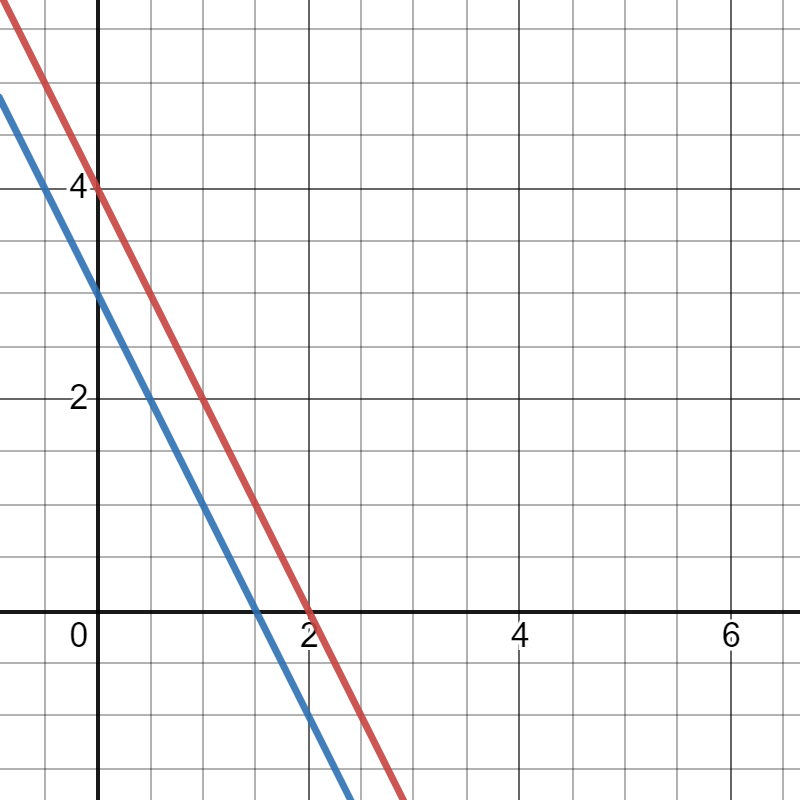
\includegraphics[width=5cm]{desmos demand shift.png}
        \end{center}
    \end{itemize}
\end{frame}

\begin{frame}{Changes in Price (cont.)}
    \begin{itemize}[<+->]
        \item However, suppose that I instead said that $y$ changed from $2$ to $1$. How do I move the curve?
        \item A: I don't. If $y=2$, then I know that we are at the point $(1,2)$ on the curve. If the $y$ value dropped to $1$, then I just move along the curve to $(1.5,1)$
        \begin{center}
            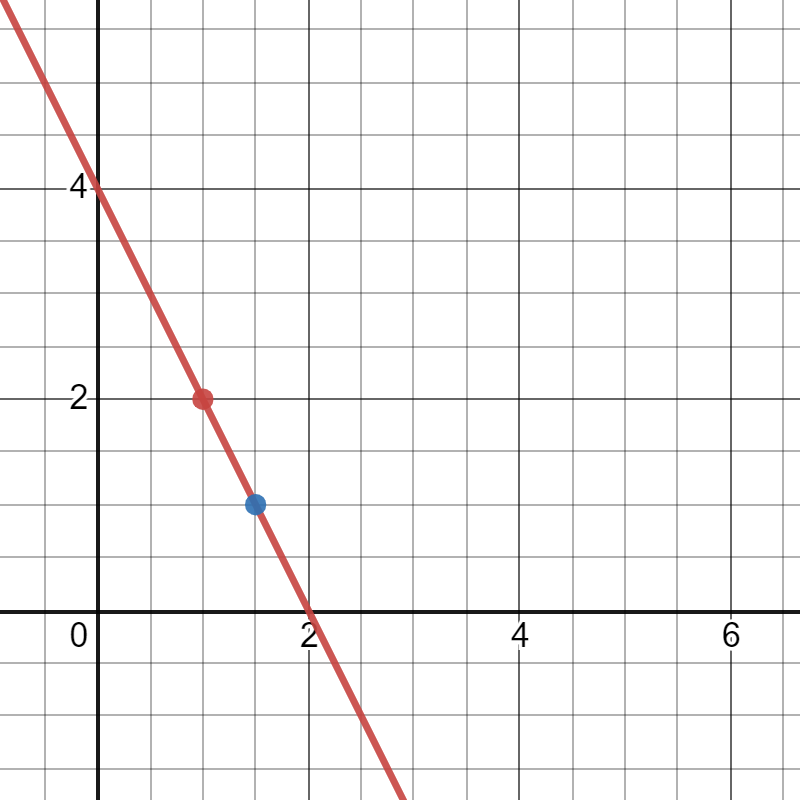
\includegraphics[width=4cm]{desmos demand along.png}
        \end{center}
    \end{itemize}
\end{frame}

\begin{frame}{Changes in Price (cont.)}
    \begin{itemize}
        \item Put another way, if I write demand as $P=-2Q+4$, and tell you that the price is $P=\$2$:
        \begin{table}[H]
            \centering
            \begin{tabular}{cc}
                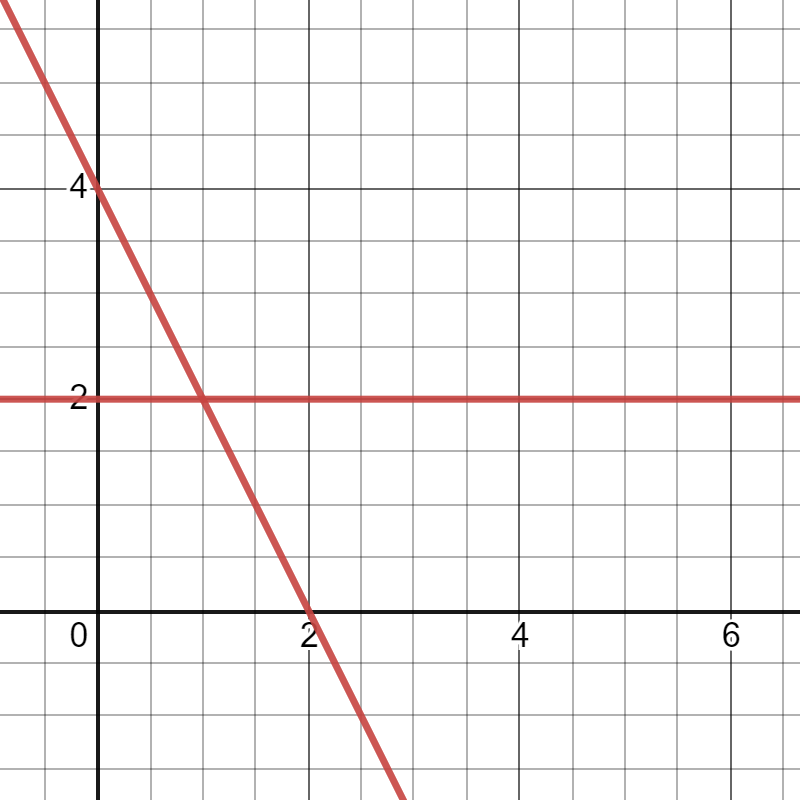
\includegraphics[width=4.5cm]{desmos demand w price.png} &\pause
                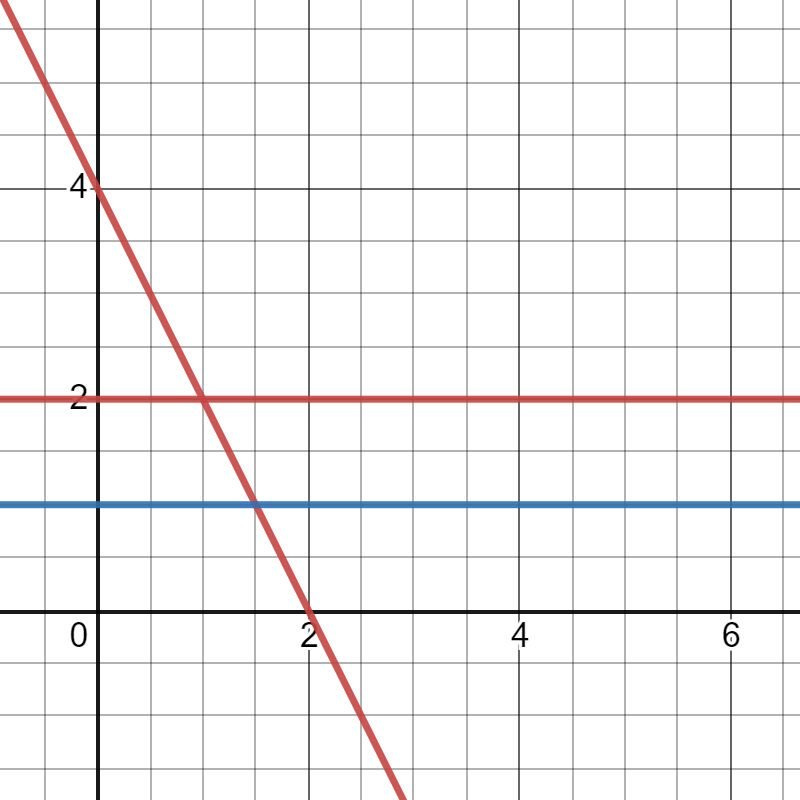
\includegraphics[width=4.5cm]{desmos demand w prices.png}
            \end{tabular}
        \end{table}
        \item<2-> Then changing the price (to $P=1$) will just cause us to move from the one intersection point to the other\footnote{\vspace{2mm}To be clear, we will never write the horizontal price lines (with the exception of ceilings/floors), they are just for illustration}
    \end{itemize}
\end{frame}

\begin{frame}{Summary of Demand Shifts}
    \begin{center}
        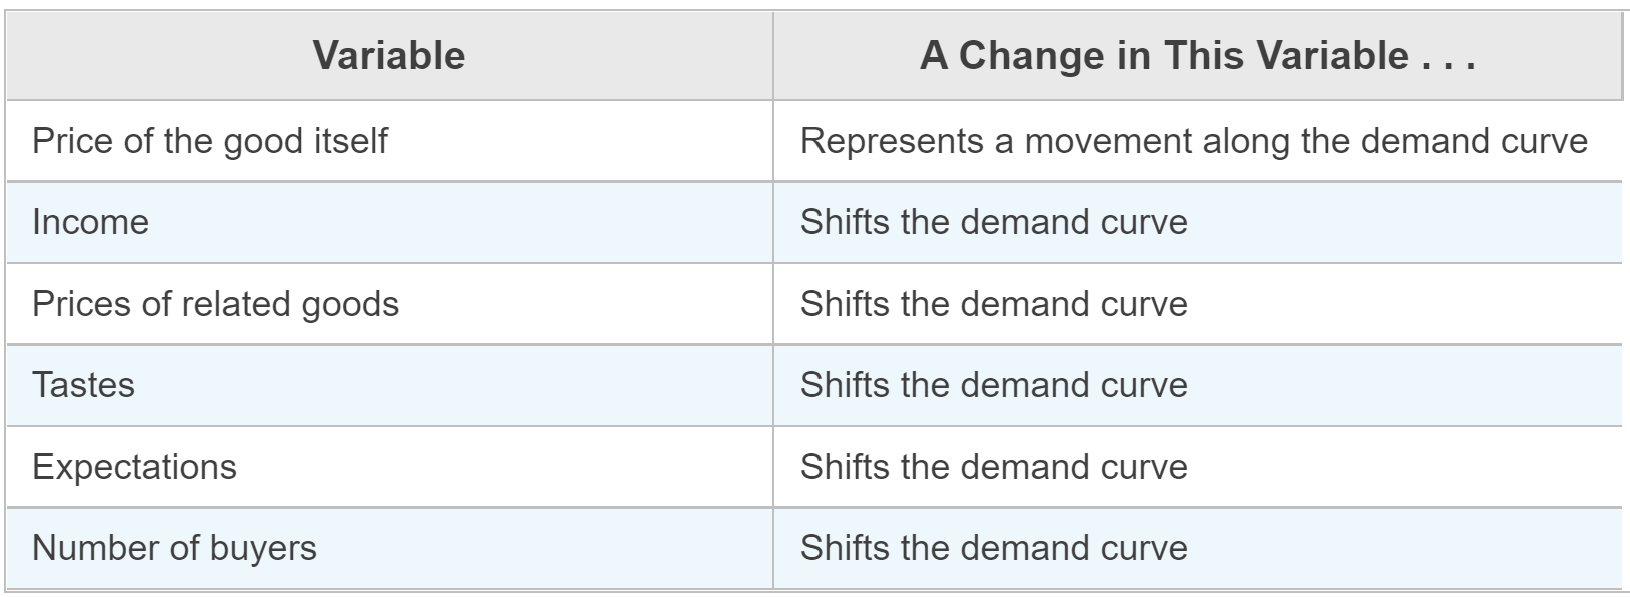
\includegraphics[width=7cm]{demand shifters table.png}
    \end{center}
    \begin{itemize}
        \item When demand shifts, it is best to say that ``the demand curve shifts" or that ``demand shifts"
        \item When there is a movement along the curve, it you should make this clear by saying something to the effect of a ``movement along the demand curve", or you can say that quantity demanded goes up or down (but you should make clear that you mean a movement not a curve shift)
        \item In short, do not say in either case that ``demand moves", be clear about what you mean, and use the terminology presented; otherwise I will assume you do not know what you are talking about
    \end{itemize}
\end{frame}

\begin{frame}{Exercise 1}
    \begin{itemize}[<+->]
        \item Suppose that the market demand curve for cereal is given by
        $$6Q+3P=18$$
        Graph the demand curve and show what would happen if the price of cereal changed from \$2 to \$5. What is the quantity demanded?
        \item \hyperlink{Sol1}{\alert{Solution}}
    \end{itemize}
\end{frame}


\begin{frame}{Exercise 2}
    \begin{itemize}[<+->]
        \item Suppose that Chad and Brad are the only people who listen to Drake albums anymore. Their demand schedules are given by
        \begin{table}[H]
            \centering
            \begin{tabular}{c|c|c}
                $P$ & $Q_{C}$ & $Q_{B}$ \\
                \hline
                \$0 & 20 & 25\\
                \$5 & 10 & 15\\
                \$8 & 8 & 9\\
                \$10 & 5 & 6\\
                \$12 & 3 & 4\\
                \$15 & 2 & 3\\
                \$20 & 0 & 2
            \end{tabular}
        \end{table}
        Graph their individual demand curves and the market demand curve. Fill in the above table with the market demand values
        \item \hyperlink{Sol2}{\alert{Solution}}
    \end{itemize}
\end{frame}

\begin{frame}{Exercise 3}
    \begin{itemize}[<+->]
        \item Suppose that Angela and Maria both have demand curves given by 
        \begin{align*}
            A: q_{a}+\frac{1}{3}P=2\\
            M: 6q_{m}=-\frac{4}{6}P+8
        \end{align*}
        Construct the equation for market demand. Write it as $P$ in terms of $Q$
        \item \hyperlink{Sol3}{\alert{Solution}}
    \end{itemize}
\end{frame}


\begin{frame}{Exercise 4}
    \begin{itemize}[<+->]
        \item Suppose that demand for coffee is given by $P=\frac{1}{Q}$:
        \begin{center}
            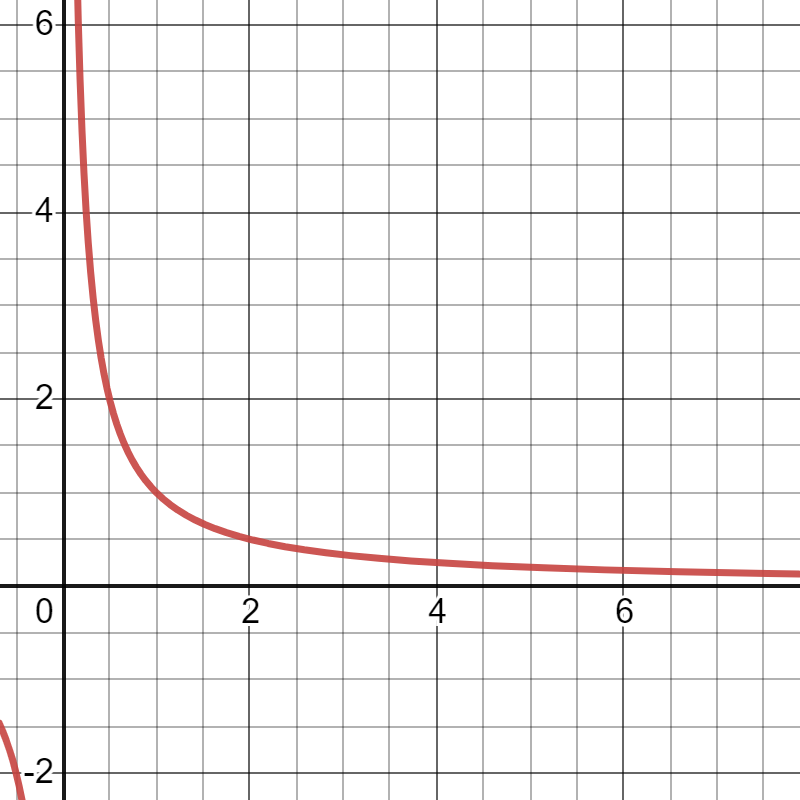
\includegraphics[width=5cm]{desmos 1-x.png}
        \end{center}
        \item If the price of creamer falls, show what happens to the demand for coffee
        \begin{itemize}
            \item<2-> If there is a movement along the curve, you may draw it however you like
            \item<2-> If the curve shifts, shift it either 1 unit to the right or 1 unit to the left
        \end{itemize}
        \item \hyperlink{Sol4}{\alert{Solution + Bonus Activity}}
    \end{itemize}
\end{frame}


\begin{frame}{Solution 1}
    \begin{itemize}
        \item Solve for $P$ in terms of $Q$: 
        $$P=-2Q+6$$
        Then we move from the red point to the blue point in the following figure:
        \begin{center}
            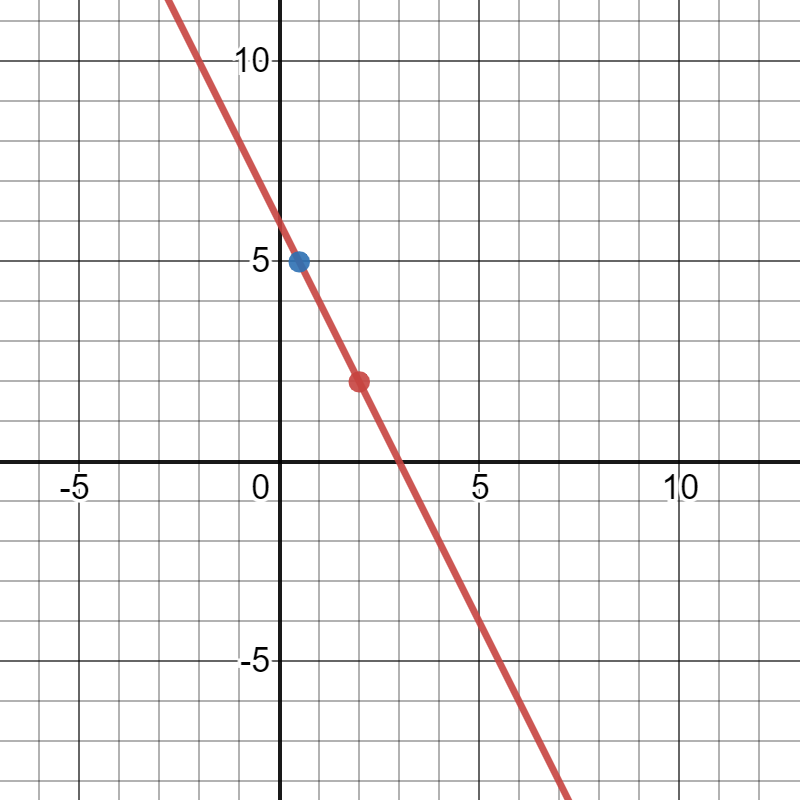
\includegraphics[width=4.5cm]{desmos ex1.png}
        \end{center}
        The new quantity demanded is 0.5 units
    \end{itemize}
    \label{Sol1}
\end{frame}

\begin{frame}{Solution 2}
    \begin{itemize}
        \item Horizontally add the individual quantities demanded. The graph should look as follows
            \begin{table}[h]
            \centering
            \begin{tabular}{c|c|c||cc}
                $P$ & $Q_{C}$ & $Q_{B}$ & $Q_{M}$ &\multirow{8}{*}{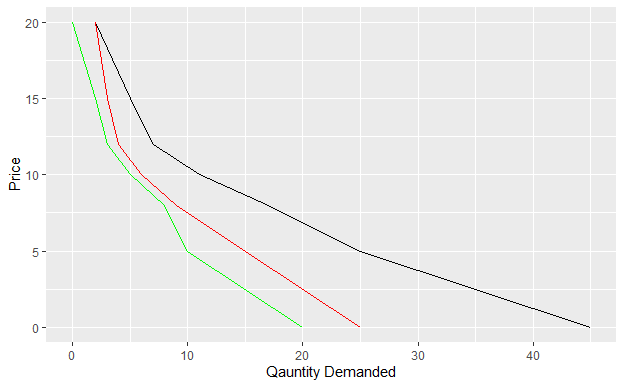
\includegraphics[width=5.5cm]{r ex2.png}}\\
                \cline{1-4}
                \$0 & 20 & 25 &45 \\
                \$5 & 10 & 15 &25\\
                \$8 & 8 & 9 & 17\\
                \$10 & 5 & 6 &11\\
                \$12 & 3 & 4 &7\\
                \$15 & 2 & 3 &6\\
                \$20 & 0 & 2 &2
            \end{tabular}
        \end{table}
    \end{itemize}
    \label{Sol2}
\end{frame}

\begin{frame}{Solution 3}
    \begin{itemize}
        \item Solve both equations for $q$:
            \begin{align*}
            A: q_{a}=-\frac{1}{3}P+2\\
            M: q_{m}=-\frac{1}{9}P+\frac{4}{3}
        \end{align*}
        \item Adding the quantities (never add prices) gets you the equation 
        $$Q=q_{a}+q_{m}=-\frac{4}{9}P+\frac{10}{3}$$
        Which can be solved to be 
        $$P=-\frac{9}{4}Q+\frac{15}{2}$$
    \end{itemize}
    \label{Sol3}
\end{frame}

\begin{frame}{Solution 4}
    \begin{itemize}
        \item The curve shifts to the right, since coffee and creamer are compliments
        \item As a math refresher, since we are given that the shift occurs by one unit, we know that the new demand curve is described by $P=\frac{1}{Q-1}$:
        \begin{center}
            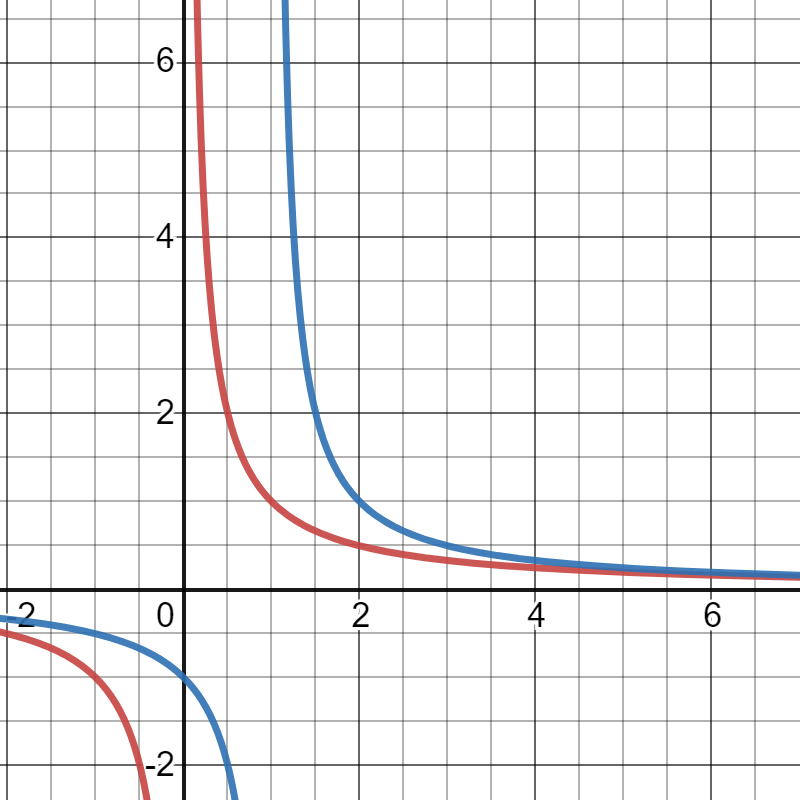
\includegraphics[width=3cm]{desmos 1-x shift.png}
        \end{center}
        \item As a bonus\footnote{Email me if you would like help with this, or to verify your answer}, graph what it would look like if I had said 1 unit up/down instead
        \item Also do this if I had said demand shifts either 1 unit up \& 1 unit right or it shifts 1 unit left \& 1 unit down. What is the equation for the graph in this case?
    \end{itemize}
    \label{Sol4}
\end{frame}

\end{document}